\sect{Конструкторский раздел}
\label{cha:C}

В данном разделе приведена диаграмма проектируемой базы данных, описана ролевая модель и хранимая процедура базы данных.

%=====================================================================
\subsect{Описание сущностей базы данных}
Исходя из формализации данных, приведенной в подразделе~\ref{cha:A-entity}, база данных должна состоять из следующих таблиц:
\begin{itemize}
	\item parkings -- таблица парковок;
	\item auto\_owners -- таблица автовладельцев (пользователей);
	\item bookings -- таблица броней;
	\item tickets -- таблица парковочных талонов;
	\item cars -- таблица машин;
	\item subscriptions -- таблица абонементов;
	\item tariffs -- таблица парковочных тарифов;
	\item parking\_meters -- таблица паркоматов;
	\item employees -- таблица сотрудников;
	\item jobs -- таблица должностей;
\end{itemize}

На рисунке~\ref{fig:DB_diagram} представлена ER-диаграмма базы данных.

\begin{figure}[h]
	\centering
	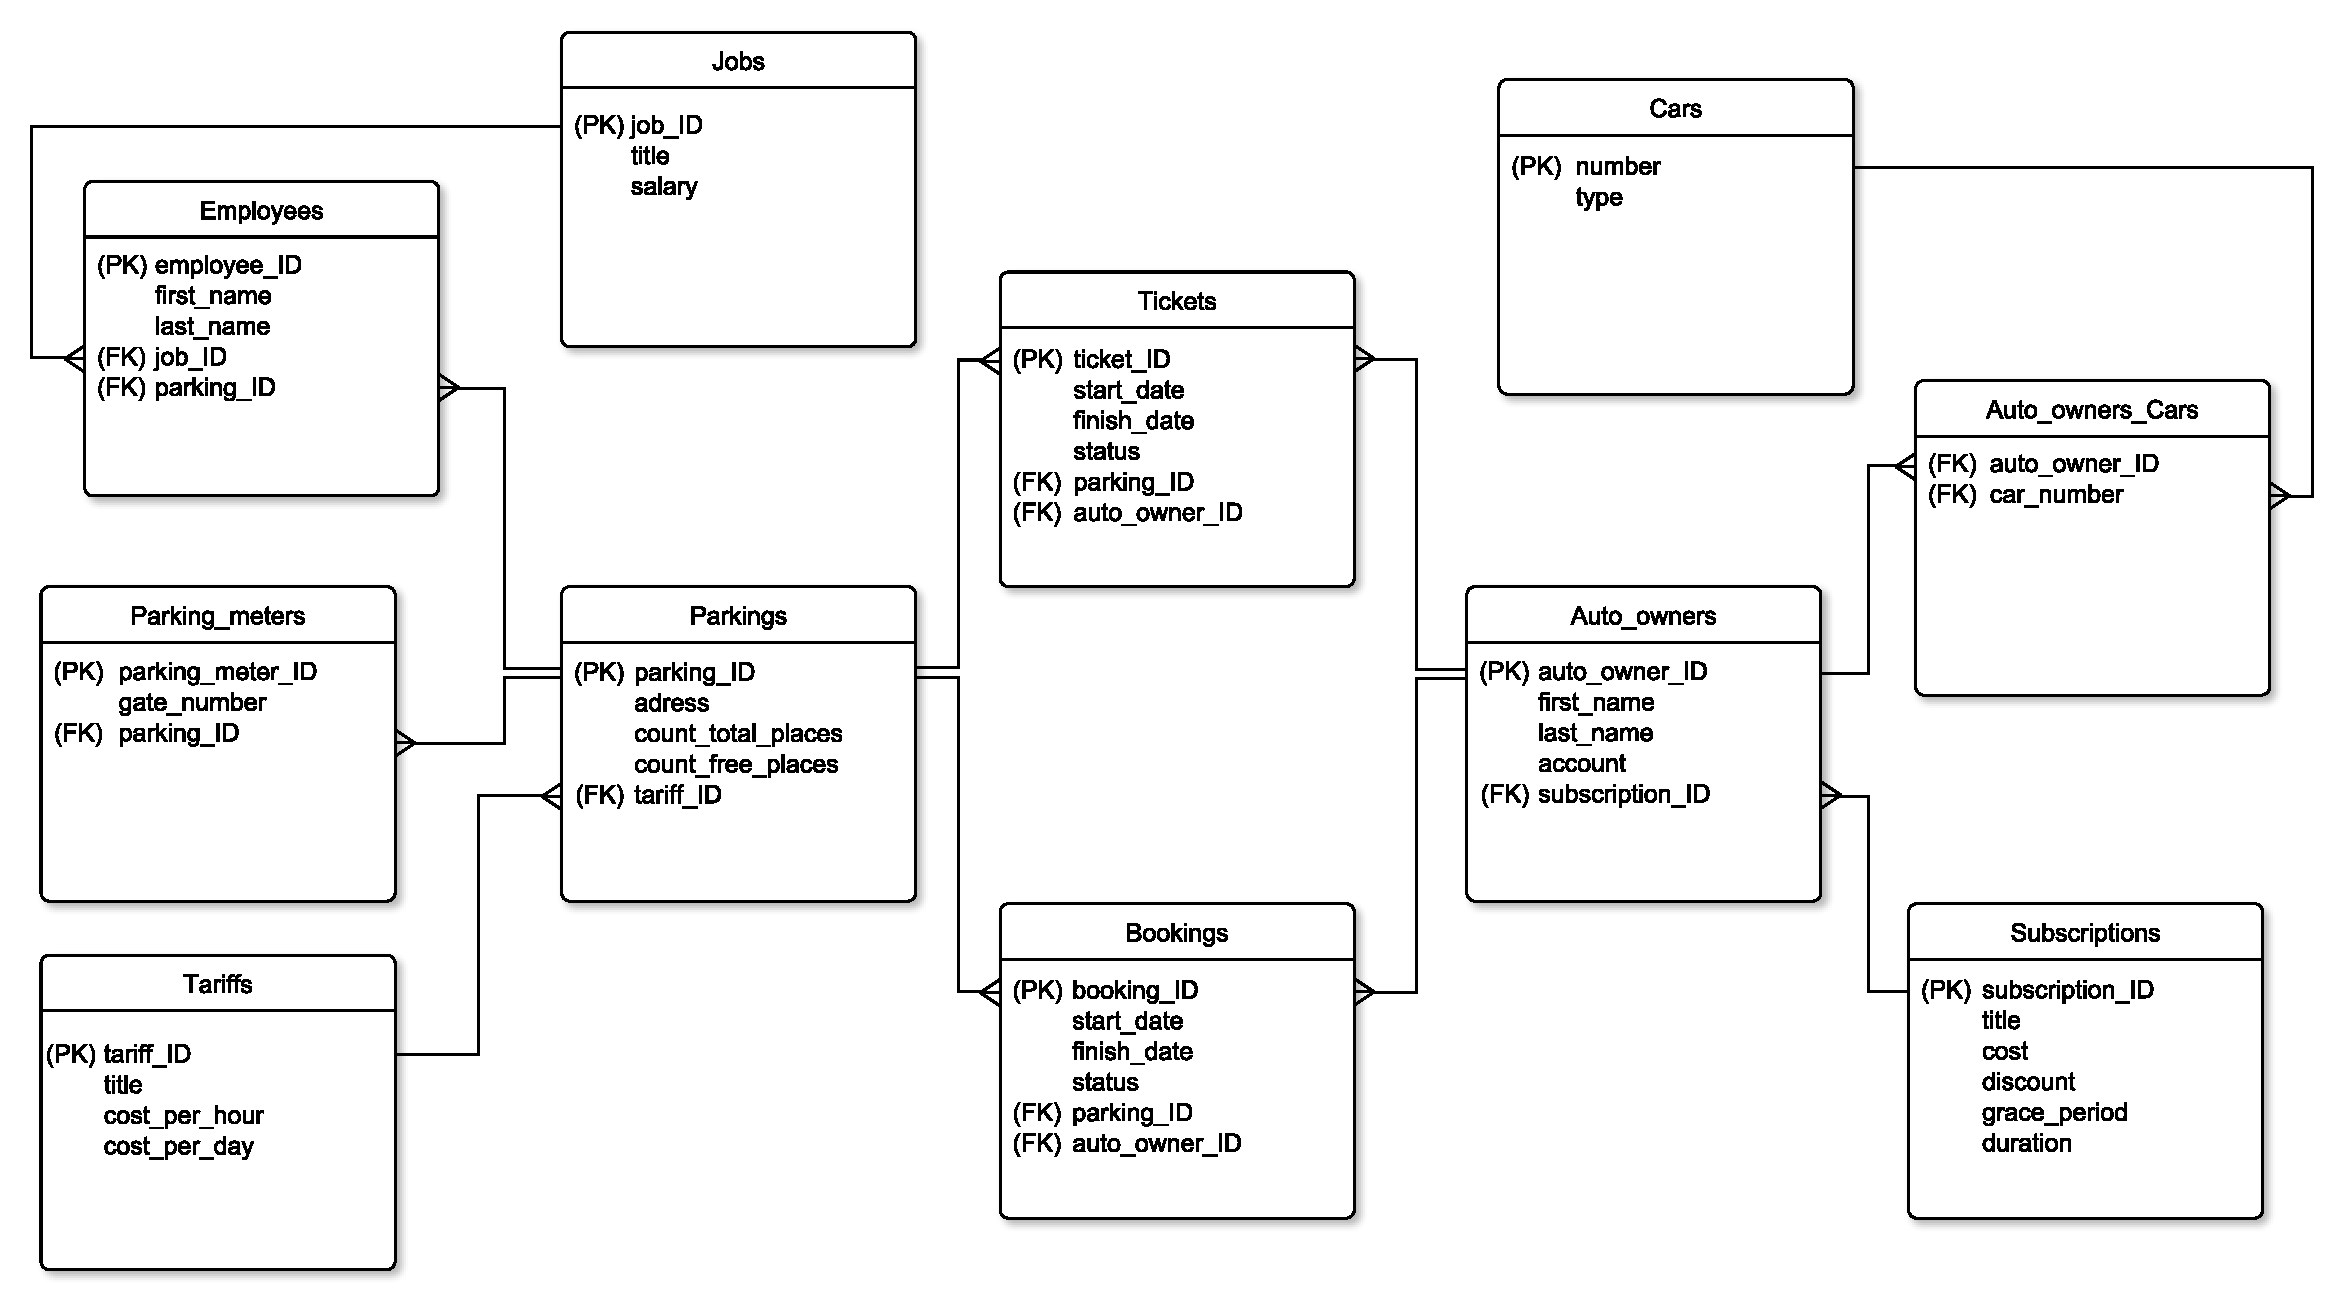
\includegraphics[width=1\textwidth, height=0.4\textheight]{svg/DB_diagram}
	%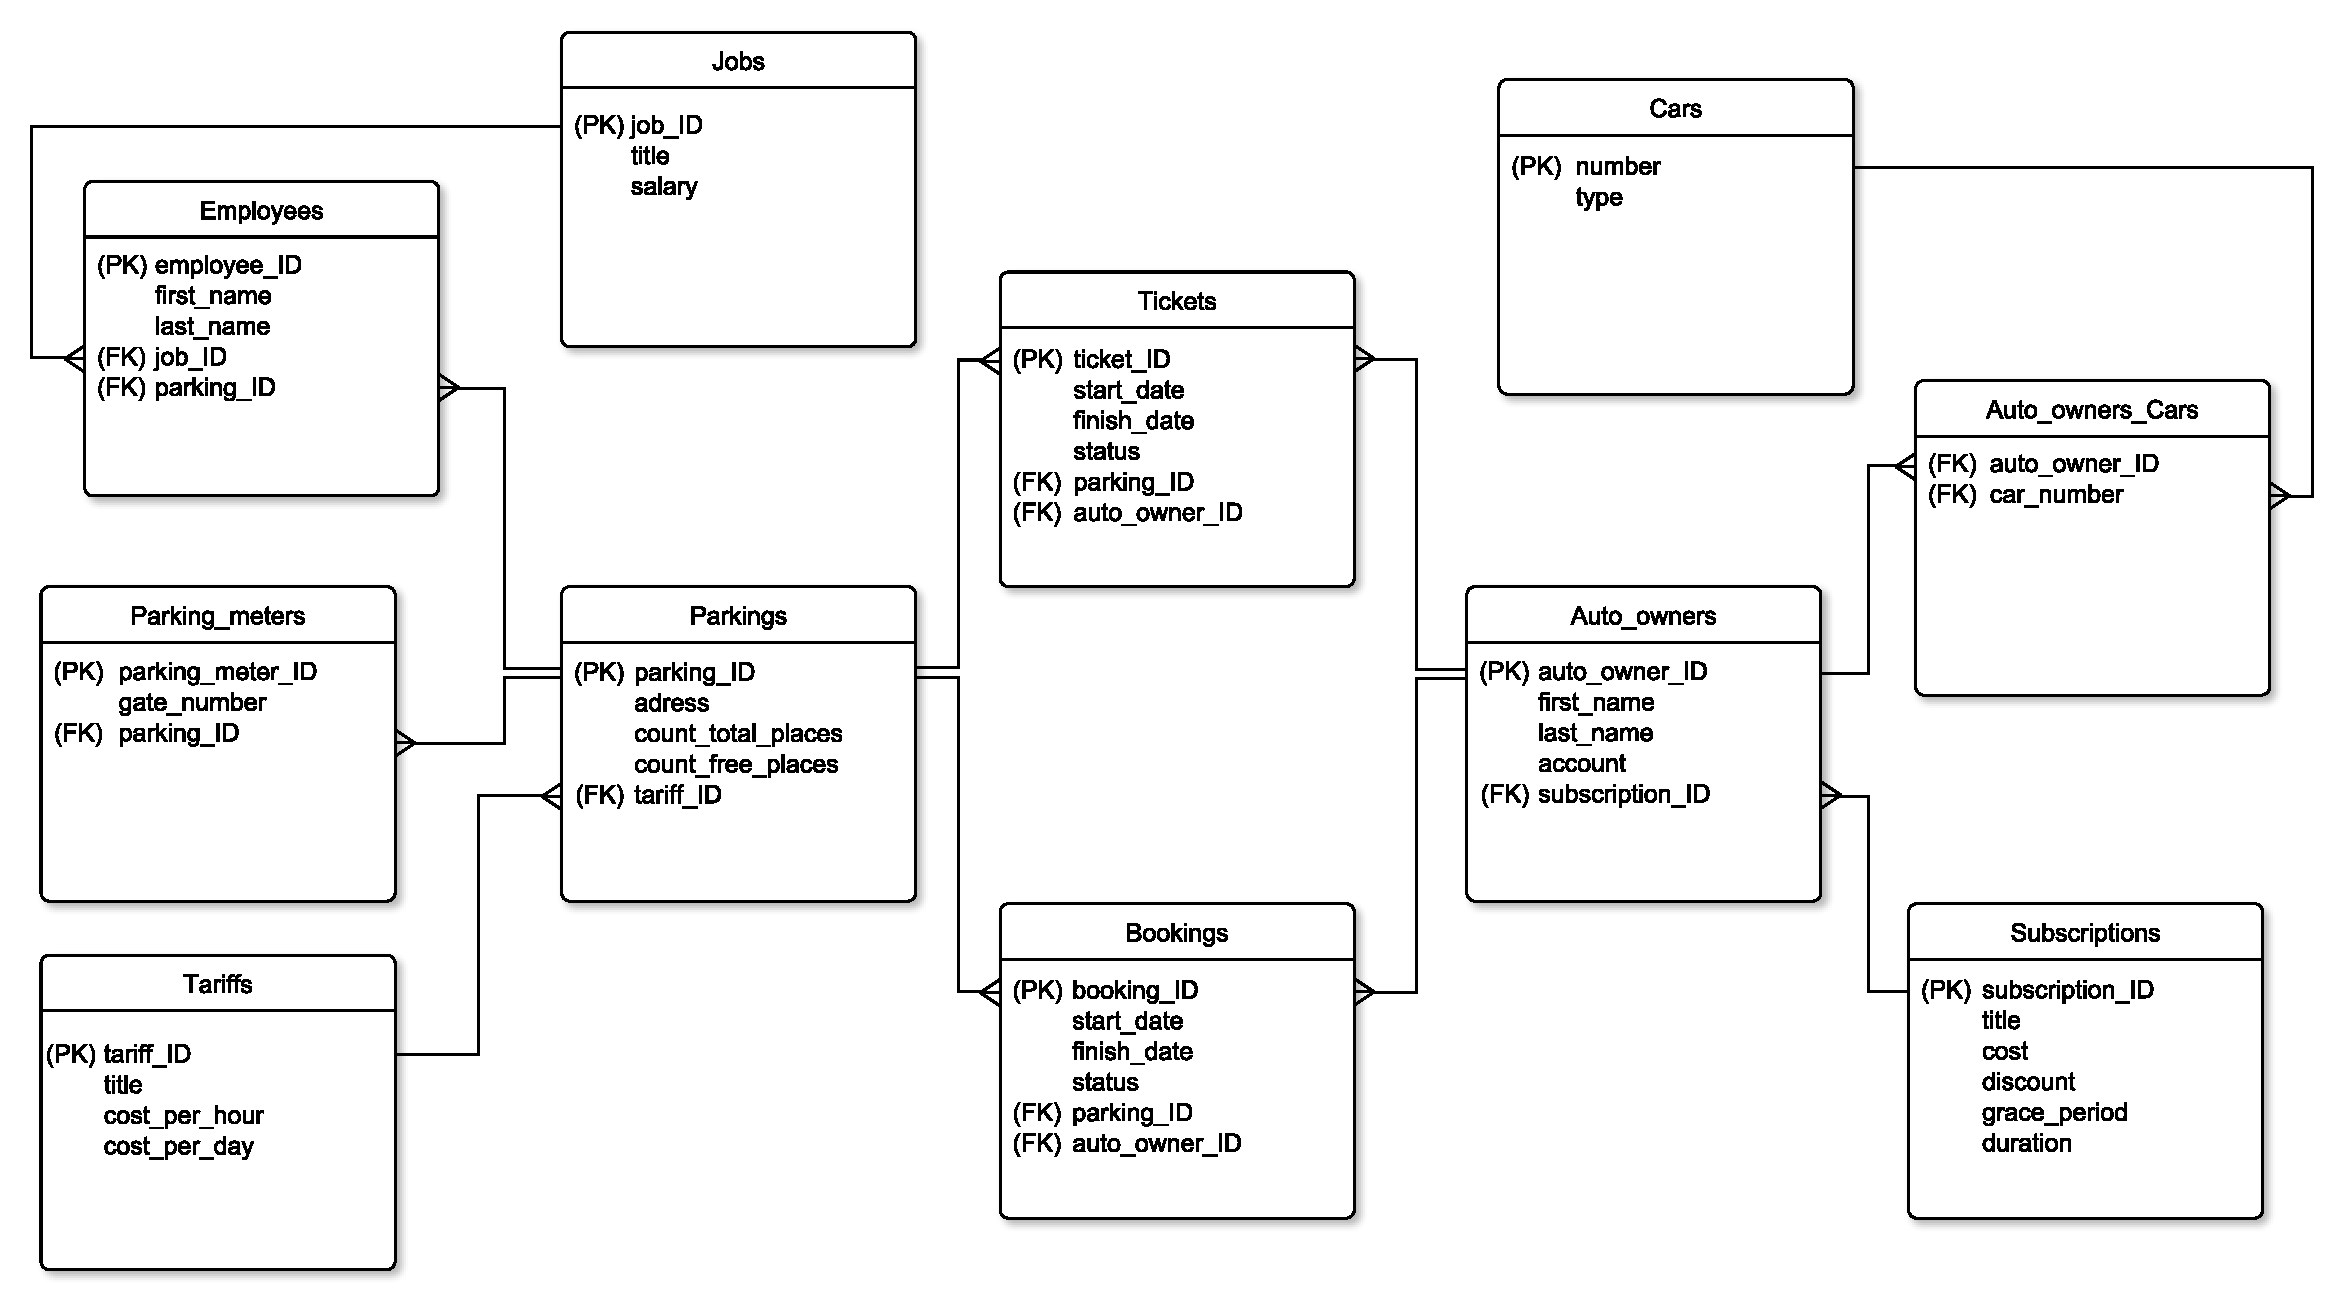
\includegraphics[height=0.5\textheight, width=0.7\textwidth]{svg/DB_diagram}
	\caption{ER-диаграмма базы данных}
	\label{fig:DB_diagram}
\end{figure}

В связи с тем, что один и тот же автомобиль может принадлежать нескольким пользователям, и при этом у одного пользователя может быть несколько автомобилей, таблицы cars и auto\_owners  находятся в отношении многие-ко-многим. Для реализации такой связи была введена таблица-связка auto\_owners\_cars.

Информация о структуре и ограничениях каждой из перечисленных таблиц указана в таблицах~\ref{tab:users}~--~\ref{tab:tickets}.

\begin{table}[H]
	\begin{center}
		\begin{center}
			\caption{\label{tab:users}Инормация о таблице auto\_owners}
		\end{center}
		\begin{tabular}{|c|c|p{3cm}|p{4cm}|}
			\hline 
			Столбец & Тип данных & Ограничение & Описание \\ \hline
			auto\_owner\_ID & INT & NOT NULL, PRIMARY KEY & Идентификатор
пользователя \\ \hline
	        first\_name &  VARCHAR(32)  & NOT NULL & Имя  \\ \hline
	        last\_name &  VARCHAR(32) & NOT NULL & Фамилия  \\ \hline
	        account & INT & NOT NULL, \( \geq 0\) & Счет  \\ \hline
	        subscription\_ID & INT & FOREIGN KEY & Идентификатор абонемента \\ \hline
		\end{tabular}
	\end{center}
\end{table}

%;;;;;;;;;;;;;;;;;;;;;;;;;;;;;;;;;;;;;;;;;;;;;;;;;;;;;;;;;;;;;;;;;;;
\begin{table}[H]
	\begin{center}
		\begin{center}
			\caption{\label{tab:aoc}Инормация о таблице auto\_owner\_cars}
		\end{center}
		\begin{tabular}{|c|c|p{3cm}|p{4cm}|}
			\hline 
			Столбец & Тип данных & Ограничение & Описание \\ \hline
	        auto\_owner\_ID & INT & NOT NULL, FOREIGN KEY & Идентификатор
пользователя  \\ \hline
	        car\_number & VARCHAR(32) & NOT NULL, FOREIGN KEY & Номер авто \\ \hline
		\end{tabular}
	\end{center}
\end{table}

%;;;;;;;;;;;;;;;;;;;;;;;;;;;;;;;;;;;;;;;;;;;;;;;;;;;;;;;;;;;;;;;;;;;
\begin{table}[H]
	\begin{center}
		\begin{center}
			\caption{\label{tab:cars}Инормация о таблице cars}
		\end{center}
		\begin{tabular}{|c|c|p{3cm}|p{4cm}|}
			\hline 
			Столбец & Тип данных & Ограничение & Описание \\ \hline
			number & VARCHAR(32) & NOT NULL, PRIMARY KEY & Номер авто \\ \hline
	        model &  VARCHAR(32)  & NOT NULL & Модель авто  \\ \hline
		\end{tabular}
	\end{center}
\end{table}

%;;;;;;;;;;;;;;;;;;;;;;;;;;;;;;;;;;;;;;;;;;;;;;;;;;;;;;;;;;;;;;;;;;;
\begin{table}[H]
	\begin{center}
		\begin{center}
			\caption{\label{tab:subs}Инормация о таблице subscriptions}
		\end{center}
		\begin{tabular}{|c|c|p{3cm}|p{4cm}|}
			\hline 
			Столбец & Тип данных & Ограничение & Описание \\ \hline
			subscription\_ID & INT & NOT NULL, PRIMARY KEY & Идентификатор
абонемента \\ \hline
	        title &  VARCHAR(32)  & NOT NULL & Название  \\ \hline
	        discount &  FLOAT & NOT NULL,\( \geq 0\), <~1 & Скидка  \\ \hline
	        cost & INT & NOT NULL, >~0 & Стоимость  \\ \hline
	        grace\_period & INT & NOT NULL,\( \geq 0\) & Льготные часы \\ \hline
	        duration & INTERVAL & NOT NULL & Срок действия абонемента \\ \hline
		\end{tabular}						 
	\end{center}
\end{table}

%;;;;;;;;;;;;;;;;;;;;;;;;;;;;;;;;;;;;;;;;;;;;;;;;;;;;;;;;;;;;;;;;;;;
\begin{table}[H]
	\begin{center}
		\begin{center}
			\caption{\label{tab:parkings}Инормация о таблице parkings}
		\end{center}
		\begin{tabular}{|c|c|p{3cm}|p{4cm}|}
			\hline 
			Столбец & Тип данных & Ограничение & Описание \\ \hline
			parking\_ID & INT & NOT NULL, PRIMARY KEY & Идентификатор
парковки \\ \hline
	        adress &  VARCHAR(32)  & NOT NULL & Адрес  \\ \hline
	        cnt\_total\_places &  INT & NOT NULL, >~0 & Количество мест всего \\ \hline
	        cnt\_free\_places & INT & NOT NULL, \( \geq 0\) & Количество свободных мест  \\ \hline
	        tariff\_ID & INT & NOT NULL, FOREIGN KEY & Идентификатор тарифа \\ \hline
		\end{tabular}
	\end{center}
\end{table}

%;;;;;;;;;;;;;;;;;;;;;;;;;;;;;;;;;;;;;;;;;;;;;;;;;;;;;;;;;;;;;;;;;;;
\begin{table}[H]
	\begin{center}
		\begin{center}
			\caption{\label{tab:tariffs}Инормация о таблице tariffs}
		\end{center}
		\begin{tabular}{|c|c|p{3cm}|p{4cm}|}
			\hline 
			Столбец & Тип данных & Ограничение & Описание \\ \hline
			tariff\_ID & INT & NOT NULL, PRIMARY KEY & Идентификатор тарифа \\ \hline
	        title &  VARCHAR(32)  & NOT NULL & Название  \\ \hline
	        cost\_per\_hour & INT & NOT NULL, \( \geq 0\) & Стоимость часа  \\ \hline
		\end{tabular}
	\end{center}
\end{table}

%;;;;;;;;;;;;;;;;;;;;;;;;;;;;;;;;;;;;;;;;;;;;;;;;;;;;;;;;;;;;;;;;;;;
\begin{table}[H]
	\begin{center}
		\begin{center}
			\caption{\label{tab:pm}Инормация о таблице parking\_meters}
		\end{center}
		\begin{tabular}{|c|c|p{3cm}|p{4cm}|}
			\hline 
			Столбец & Тип данных & Ограничение & Описание \\ \hline
			parking\_meter\_ID & INT & NOT NULL, PRIMARY KEY & Идентификатор паркомата \\ \hline
	        gate\_number & INT & NOT NULL, \( \geq 0\) & Номер въезда  \\ \hline
	        parking\_ID & INT & NOT NULL, FOREIGN KEY & Идентификатор парковки \\ \hline
		\end{tabular}
	\end{center}
\end{table}

%;;;;;;;;;;;;;;;;;;;;;;;;;;;;;;;;;;;;;;;;;;;;;;;;;;;;;;;;;;;;;;;;;;;
\begin{table}[H]
	\begin{center}
		\begin{center}
			\caption{\label{tab:empl}Инормация о таблице employees}
		\end{center}
		\begin{tabular}{|c|c|p{3cm}|p{4cm}|}
			\hline 
			Столбец & Тип данных & Ограничение & Описание \\ \hline
			employee\_ID & INT & NOT NULL, PRIMARY KEY & Идентификатор
сотрудника \\ \hline
	        first\_name &  VARCHAR(32)  & NOT NULL & Имя  \\ \hline
	        last\_name &  VARCHAR(32) & NOT NULL & Фамилия  \\ \hline
	        job\_ID & INT & NOT NULL, FOREIGN KEY & Идентификатор должности \\ \hline
	        parking\_ID & INT & NOT NULL, FOREIGN KEY & Идентификатор парковки \\ \hline
		\end{tabular}
	\end{center}
\end{table}

%;;;;;;;;;;;;;;;;;;;;;;;;;;;;;;;;;;;;;;;;;;;;;;;;;;;;;;;;;;;;;;;;;;;
\begin{table}[H]
	\begin{center}
		\begin{center}
			\caption{\label{tab:jobs}Инормация о таблице jobs}
		\end{center}
		\begin{tabular}{|c|c|p{3cm}|p{4cm}|}
			\hline 
			Столбец & Тип данных & Ограничение & Описание \\ \hline
			job\_ID & INT & NOT NULL, PRIMARY KEY & Идентификатор должности \\ \hline
	        title &  VARCHAR(32)  & NOT NULL & Название  \\ \hline
	        salary &  INT & NOT NULL, > 0 & Оклад  \\ \hline
		\end{tabular}
	\end{center}
\end{table}

%;;;;;;;;;;;;;;;;;;;;;;;;;;;;;;;;;;;;;;;;;;;;;;;;;;;;;;;;;;;;;;;;;;;
\begin{table}[H]
	\begin{center}
		\begin{center}
			\caption{\label{tab:bookings}Инормация о таблице bookings}
		\end{center}
		\begin{tabular}{|c|c|p{3cm}|p{4cm}|}
			\hline 
			Столбец & Тип данных & Ограничение & Описание \\ \hline
			booking\_ID & INT & NOT NULL, PRIMARY KEY & Идентификатор брони \\ \hline
	        start\_date & TIMESTAMP  & NOT NULL & Дата начала  \\ \hline
	        finish\_date &  TIMESTAMP & >~start\_date & Дата окончания  \\ \hline
	        status & BOOLEAN & NOT NULL & Статус \\ \hline
	        parking\_ID & INT & NOT NULL, FOREIGN KEY & Идентификатор парковки \\ \hline
	        auto\_owner\_ID & INT & NOT NULL, PRIMARY KEY & Идентификатор пользователя \\ \hline
		\end{tabular}
	\end{center}
\end{table}

%;;;;;;;;;;;;;;;;;;;;;;;;;;;;;;;;;;;;;;;;;;;;;;;;;;;;;;;;;;;;;;;;;;;
\begin{table}[H]
	\begin{center}
		\begin{center}
			\caption{\label{tab:tickets}Инормация о таблице tickets}
		\end{center}
		\begin{tabular}{|c|c|p{3cm}|p{4cm}|}
			\hline 
			Столбец & Тип данных & Ограничение & Описание \\ \hline
			ticket\_ID & INT & NOT NULL, PRIMARY KEY & Идентификатор талона \\ \hline
	        start\_date & TIMESTAMP  & NOT NULL & Дата начала  \\ \hline
	        finish\_date &  TIMESTAMP & >~start\_date & Дата окончания  \\ \hline
	        status & BOOLEAN & NOT NULL & Статус \\ \hline
	        parking\_ID & INT & NOT NULL, FOREIGN KEY & Идентификатор парковки \\ \hline
	        auto\_owner\_ID & INT & NOT NULL, PRIMARY KEY & Идентификатор пользователя \\ \hline
		\end{tabular}
	\end{center}
\end{table}

%=====================================================================
\subsect{Ролевая модель}
Согласно диаграмме использования приложения, представленной на рисунке~\ref{fig:use_case}, необходимо выделить следующие роли:
\begin{itemize}
	\item гость -- обладает правами только на просмотр таблиц parkings, tariffs, subscriptions;
	\item автовладелец -- обладает правами на просмотр и изменение записей, связанных с ним, во всех таблицах, кроме employees, jobs и parking\_meters;
	\item паркомат -- обладает правами на просмотр всех таблиц, создание и обновление записей в таблицах bookings и tickets;
	\item Администратор -- обладает всеми правами доступа ко всем таблицам.
\end{itemize}

%=====================================================================
\subsect{Хранимая процедура}
В проектируемой базе данных таблицы cars и auto\_owners связанны отношением многие-ко-многим. 
При создании нового авто необходимо обновить сразу две таблицы: таблицу cars и таблицу-связку auto\_owners\_cars. 
Для повешения надежности и вместе с тем упрощения процесса добавления нового авто, было решено написать хранимую процедуру insert\_car, выполняющую эту задачу.

%=====================================================================
\subsect{Диаграмма классов приложения}
На рисунке~\ref{fig:uml} приведена UML-диаграмма классов.
\begin{figure}[h]
	\centering
	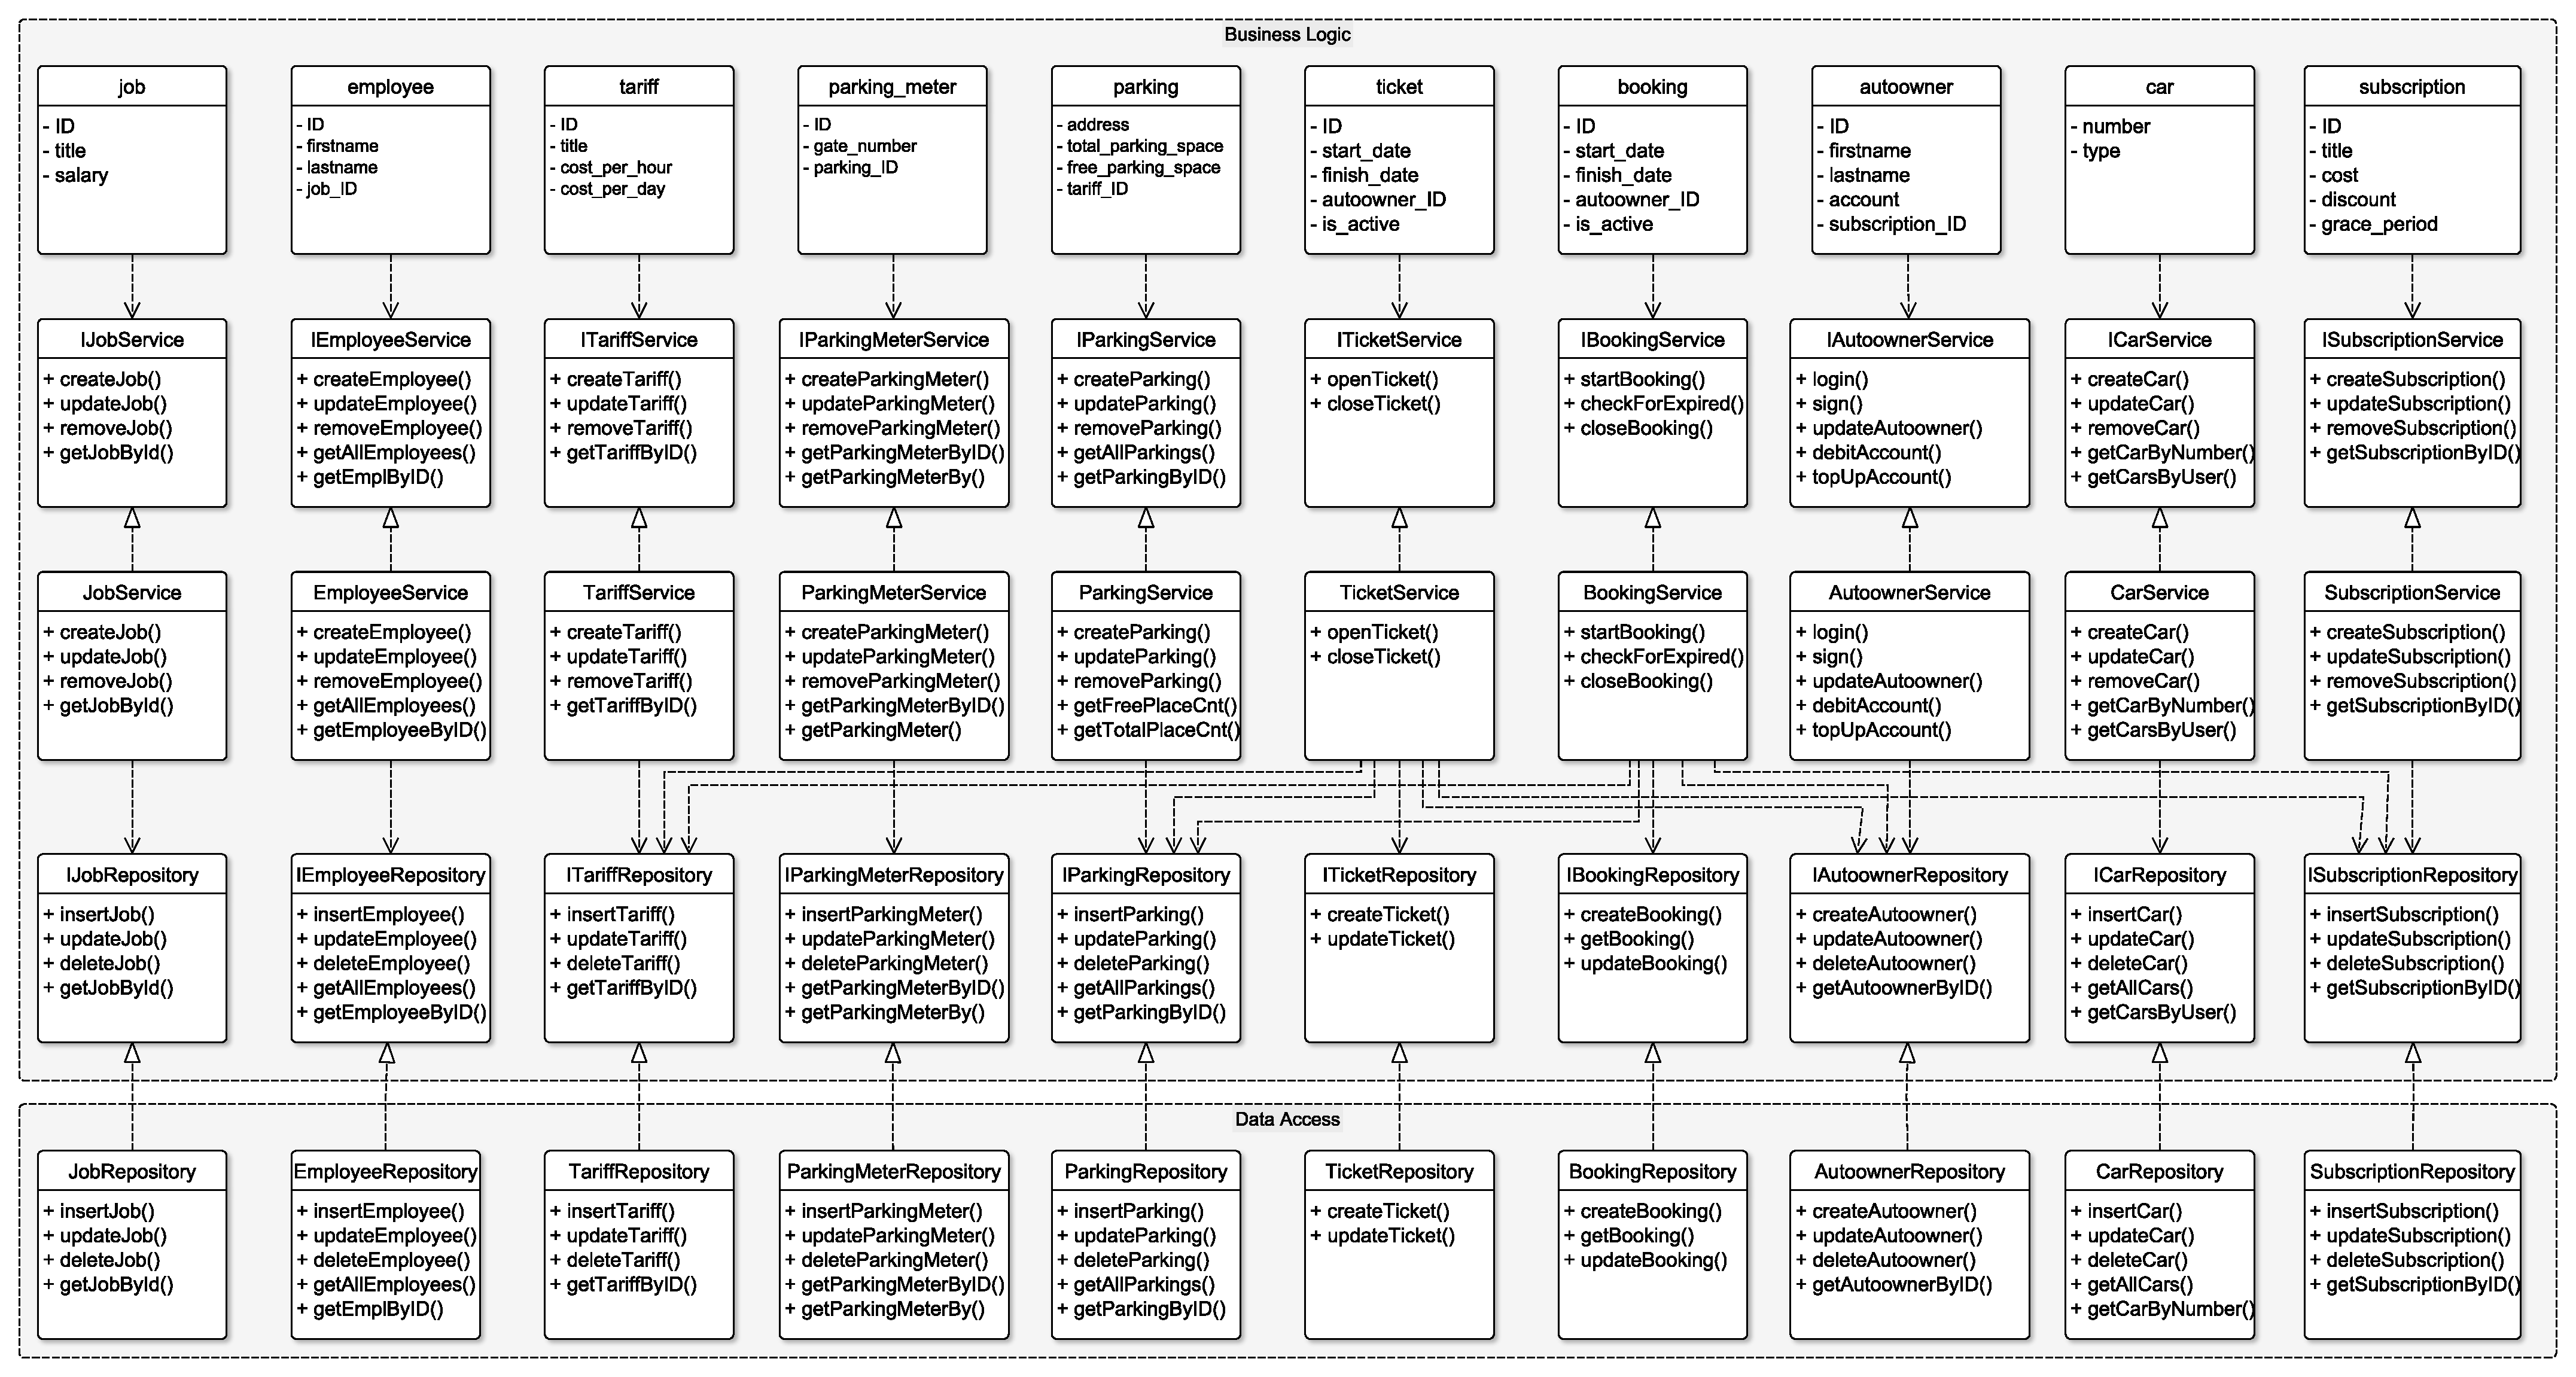
\includegraphics[height=0.6\textheight, width=1.1\textwidth, angle=90]{svg/UML}
	\caption{UML-диаграмма классов}
	\label{fig:uml}
\end{figure}

Проектирование велось в соответствии с принципами <<чистой архитектуры>>~\cite{martin}, в частности был спроектирован компонент бизнес-логики, полностью независимый от компонента доступа к данным и пользовательского интерфейса.

~

%=====================================================================
\subsect{Вывод}
В данном разделе были описаны сущности проектируемой базы данных, ролевая модель и хранимая процедура. Также приведена ER-диаграмма базы данных и UML-диаграмма классов.
